\clearpage
\section{Results}
\subsection{Random Graphs}

We compare the output of the algorithm versus the exact solution obtained by formulating the target set selection problem as an 0-1 Integer Linear Programming problem. This is to show that the algorithm also works on moderate sized graphs. 

The graphs used for this experiment are random graphs. We create a random graph $(N,p)$, $N \in N^{+}$ as the number of vertices and $p$ as the probability of how an edge between vertices appear. This experiment was done on graphs with 30 nodes and 50 nodes each done with incrementing probabilities: $p\in{10/100,20/100,...,90/100}$.

The formulation of our ILP is based of an existing model by Raghavan\cite{wtss} which is a modified version of Ackerman et.al's model\cite{combi}. Raghavan's model is for the $Weighted$ Target Set Selection problem. We can tweak the formulation by setting the weight variables as $w_{i}=1$ to fit our problem.

Integer Linear Programming is a technique for optimizing a linear objective function, subject to linear constraints. We either want to maximize or minimize an objective function based off our problem. We restrict the variables in this problem to having only values $\in {0,1}$. These variables are called decision variables.

Given a graph $G=(V,E)$, $v \in V$, $e \in E$, we assign a threshold $t_{v}$ to each node in the graph. We also define two decision variables for this formulation $x_{v}\in\{0,1\}, e_{u,v}\in\{0,1\}$. $x_{v}$ is the decision variable we want to minimize the summation. It shows that if $x_{v}=1$, we know that this vertex is selected as part of the target set. The variable $e_{(u,v)}$ indicates the direction of activation of nodes. If $e_{1,2}=1$ and $e_{2,1}=0$, it states that node 1 activated node 2 not the other around. Restricting the sum of the two variables of one edge to 1 will follow the monotonic aspect of TSS that once a node is active it will not go back to inactive\cite{wtss}. The 2nd constraint says that a node $v\in V$ must be activated or have atleast $t_{v}$ incoming edges. For identifying the minimum of the equation, we need to find the values of $x$ and $e$ such that the objective function is at a minimum but still satisfies our constraints.

The formulation is defined as:
\begin{equation*}
	\begin{aligned}
	& {\text{minimize}}&\sum_{v\in V}{x_{v}}\\ 
	&\text{subject to} & e_{u,v}+e_{v,u}=1  &&\forall\{u,v\}\in\ E \\
	& & \sum_{v\in n(v)} e_{v,u} + t_{v} x_{v}& \geq t_{v} & \forall v \in V\\
	& &x_{v} \in \{0,1\}  & & \forall v \in V\\
	& &e_{v,u}\in \{0,1\}  & & \forall v \in V\\
	\end{aligned}
\end{equation*}

We use the example from before to better understand how to formulate the problem. The example has 10 vertices and 9 edges. We use 10 $x$ variables and 18 $e$ variables. 

\begin{equation*}
	\begin{aligned}
	&&& {\text{minimize}} \ x_{1}+x_{2}+x_{3}+x_{4}+x_{5}+x_{6}+x_{7}+x_{8}+x_{9}+x_{10}&&&\\ 
	&&&\text{subject to} && \\
	&&&e_{1,2}+e_{2,1}=1&&&\\
	&&&e_{1,3}+e_{3,1}=1&&&\\
	&&&e_{1,4}+e_{4,1}=1&&&\\
	&&&e_{1,7}+e_{7,1}=1&&&\\
	&&&e_{4,5}+e_{5,4}=1&&&\\
	&&&e_{5,6}+e_{6,5}=1&&&\\
	&&&e_{6,10}+e_{10,6}=1&&&\\
	&&&e_{7,8}+e_{8,7}=1&&&\\
	&&&e_{7,9}+e_{9,7}=1&&&\\	
	&&& e_{1,2}+e_{1,3}+e_{1,4}+e_{1,7}+3x_{1}\geq 3&&&\\
	&&& e_{2,1} + x_{2}\geq 1&&&\\
	&&& e_{3,1} + x_{3}\geq 1&&&\\
	&&& e_{4,1} + e_{4,5} + x_{4}\geq 1&&&\\
	&&& e_{5,4} + e_{5,6} + 2 x_{5}\geq 2&&&\\
	&&& e_{6,5} + e_{6,10} + x_{6}\geq 1&&&\\
	&&& e_{7,1} + e_{7,8} + e_{7,9} + 2 x_{6}\geq 2&&&\\
	&&& e_{8,7} + x_{8}\geq 1&&&\\
	&&& e_{9,7} + x_{9}\geq 1&&&\\
	&&& e_{10,6} + x_{10}\geq 1&&&\\
	&& &x_{v} \in \{0,1\}  \forall v \in V&&&\\
	&& &e_{v,u}\in \{0,1\}  \forall v \in V &&&\\
	\end{aligned}
\end{equation*}

We can input these equations into a solver and we get $x_{1}=x_{5}=x_{7}=1$. The paper being studies got the same result with the TSS algorithm but the vertex selection started with the last node instead of the first node to be eligible. We get different vertices in different runs of TSS if the selection of the vertex in case 3 is random but, the cardinality stays the same.

The random graphs and ILP objective function and constraints were generated and using matlab 2017a. The ILP formulation of the random graphs was solved using \textit{LPSolve}\cite{lpsolve}. The max number of variables we generate is 1000-1200, this is for only 50 nodes and 90/100 probability.

Here are the results we get from the experiment:

\begin{figure}[h!]
\begin{minipage}[t]{0.50\textwidth}
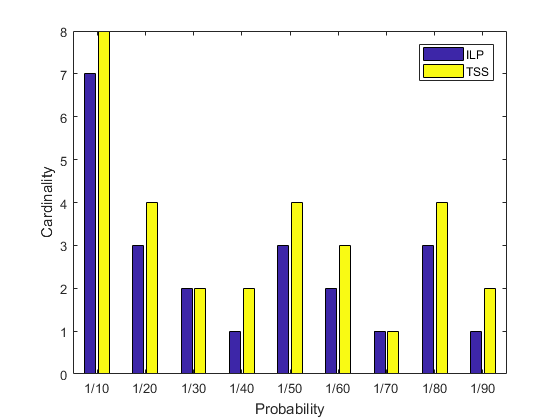
\includegraphics[width=\linewidth,keepaspectratio=true]{images/rand30result.png}
\caption{30 nodes}

\end{minipage}
\begin{minipage}[t]{0.50\textwidth}
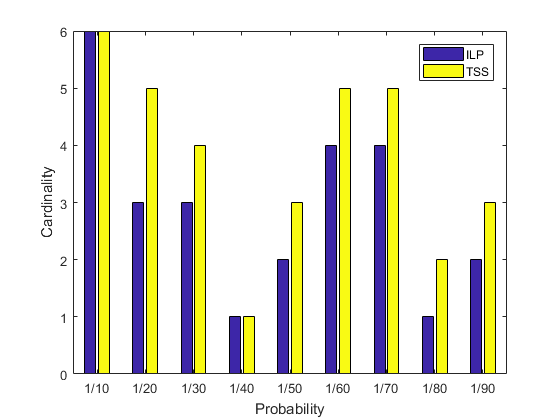
\includegraphics[width=\linewidth,keepaspectratio=true]{images/rand50result.png}
\caption{50 nodes}
\end{minipage}
\end{figure}

The data shows that the TSS algorithm produces a result that is near the exact solution and at times is the same as the exact solution for graphs with a \textit{small} amount of vertices.

\subsection{TSS applied to real-life networks}

We apply the TSS algorithm to real-life networks and compare it to the previously developed algorithm and a greedy version of TSS. The threshold of the nodes are set as $t(v)\in(1,2,...,10)$ for each iteration. For the random version of algorithms if more than one node meets the condition of cases we randomly selected a node from the set of nodes that satisfy the condition in each algorithm. The selection of nodes in case 3 of TSS can be randomized. We test if randomness of selection of nodes affect the cardinality of the target set and the runtime of the algorithm.

In this experiment we run each algorithm once for each threshold for the normal version of the algorithm and 5 times for the random version of the algorithm. That makes 10 runs per dataset. For the VirAds algorithm we experiment the amount of $d$ hops needed to output an ideal solution. This is why we run the algorithm 10 times per threshold starting with $d=1$ upto $d=10$. That makes 100 runs per dataset for the VirAds algorithm. In analyzing the data, we plot the cardinality and runtime of the network versus the thresholds that was used in obtaining them. For the data in the random runs, we average the cardinality and time then plot it against the thresholds. We then compare the normal and random amongst each other using a bar plot.

We get our data from real-life networks\cite{datasets1}\cite{datasets2}. The following datasets are used:
\begin{enumerate}
	\item BlogCatalog3 (10,312 nodes, 333,983 edges): a social blog directory which manages the bloggers and their blogs. Both the contact network and selected group membership information are included.
	\item Ca-AstroPh(18,772 nodes, 198,110 edges): Arxiv ASTRO-PH (Astro Physics) collaboration network is from the e-print arXiv and covers scientific collaborations between authors papers submitted to Astro Physics category.
	\item Ca-CondMat (23,133 nodes, 93,497 edges): Arxiv COND-MAT (Condense Matter Physics) collaboration network is from the e-print arXiv and covers scientific collaborations between authors papers submitted to Condense Matter category.
	\item Ca-GrQc (5,242 nodes, 14,496 edges): Arxiv GR-QC (General Relativity and Quantum Cosmology) collaboration network is from the e-print arXiv and covers scientific collaborations between authors papers submitted to General Relativity and Quantum Cosmology category. 
	\item Ca-HepPh (12,008 nodes, 118,521 edges): Arxiv HEP-PH (High Energy Physics - Phenomenology) collaboration network is from the e-print arXiv and covers scientific collaborations between authors papers submitted to High Energy Physics - Phenomenology category.
	\item Ca-HepTh (9,877 nodes, 25,998 edges): Arxiv HEP-TH (High Energy Physics - Theory) collaboration network is from the e-print arXiv and covers scientific collaborations between authors papers submitted to High Energy Physics - Theory category. 
	\item Douban (154907 nodes, 654188 edges):
	 Douban.com, launched on March 6, 2005, is a Chinese Web 2.0 website providing user review and recommendation services for movies, books, and music.
\end{enumerate}

\begin{figure}[h!]
\begin{minipage}[t]{0.50\textwidth}
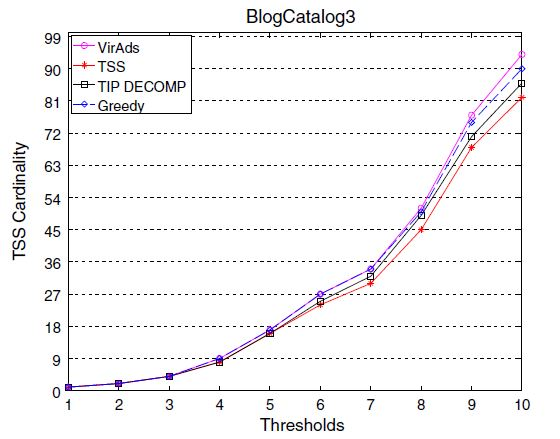
\includegraphics[width=\linewidth,keepaspectratio=true]{images/bc3paper.jpg}
\caption{Cardinality vs Threshold}
\label{fase1}
\end{minipage}
\begin{minipage}[t]{0.50\textwidth}
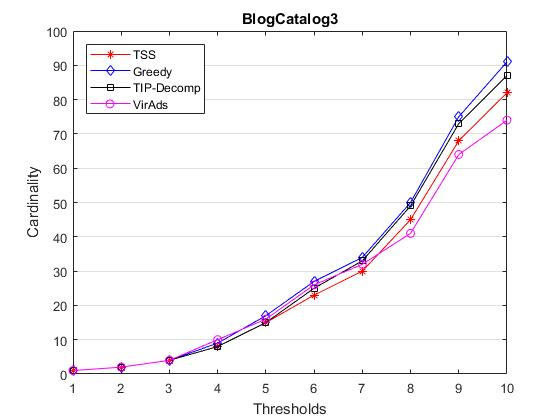
\includegraphics[width=\linewidth,keepaspectratio=true]{images/bc3result.jpg}
\caption{Cardinality vs Threshold}
\end{minipage}
\end{figure}

\begin{figure}[h!]
\begin{minipage}[t]{0.50\textwidth}
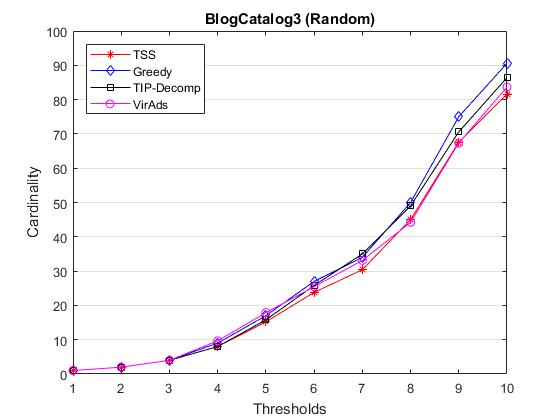
\includegraphics[width=\linewidth,keepaspectratio=true]{images/bc3resultrandom.jpg}
\caption{Time vs Threshold}

\end{minipage}
\begin{minipage}[t]{0.50\textwidth}
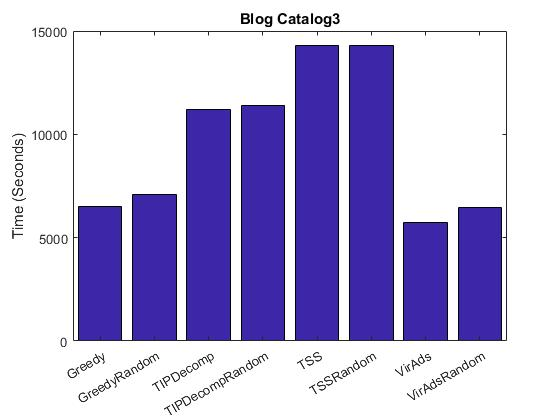
\includegraphics[width=\linewidth,keepaspectratio=true]{images/bc3time1.jpg}
\caption{Time vs Threshold}
\end{minipage}
\end{figure}

\begin{figure}[h!]
\begin{minipage}[t]{0.50\textwidth}
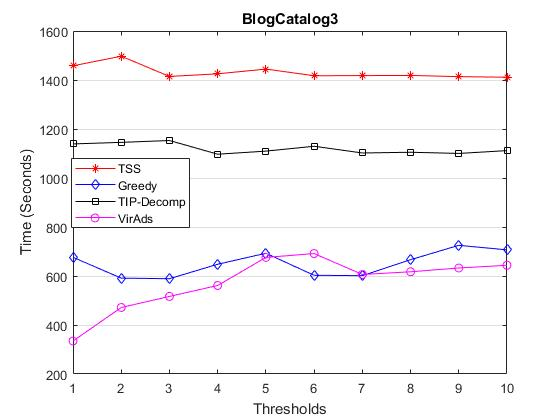
\includegraphics[width=\linewidth,keepaspectratio=true]{images/bc3time.jpg}
\caption{Time vs Threshold}

\end{minipage}
\begin{minipage}[t]{0.50\textwidth}
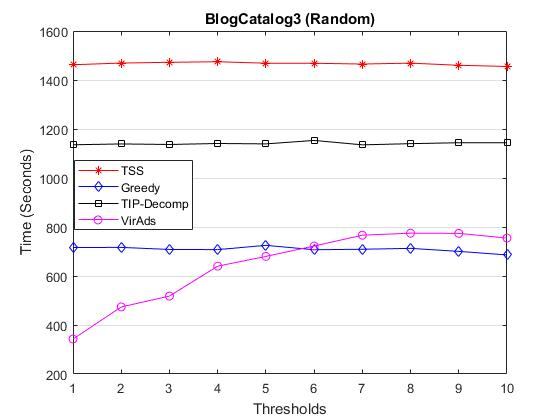
\includegraphics[width=\linewidth,keepaspectratio=true]{images/bc3timerandom.jpg}
\caption{Time vs Threshold}
\end{minipage}
\end{figure}
\begin{figure}[h!]
\begin{minipage}[t]{0.50\textwidth}
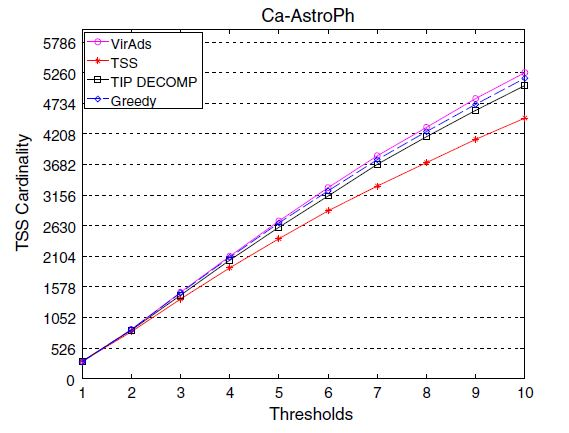
\includegraphics[width=\linewidth,keepaspectratio=true]{images/ca-astrophpaper.jpg}
\caption{Cardinality vs Threshold}

\end{minipage}
\begin{minipage}[t]{0.50\textwidth}
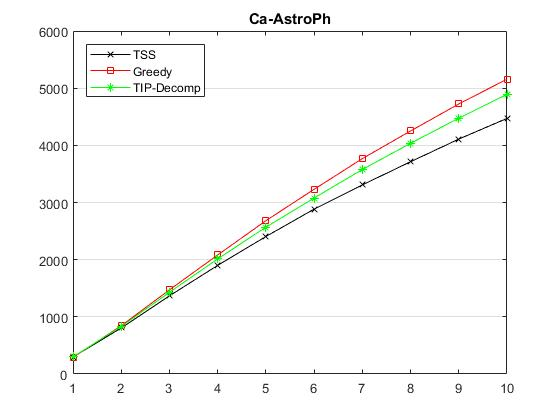
\includegraphics[width=\linewidth,keepaspectratio=true]{images/ca-astrophresult.jpg}
\caption{Cardinality vs Threshold}
\end{minipage}
\end{figure}

\begin{figure}[h!]
\begin{minipage}[t]{0.50\textwidth}
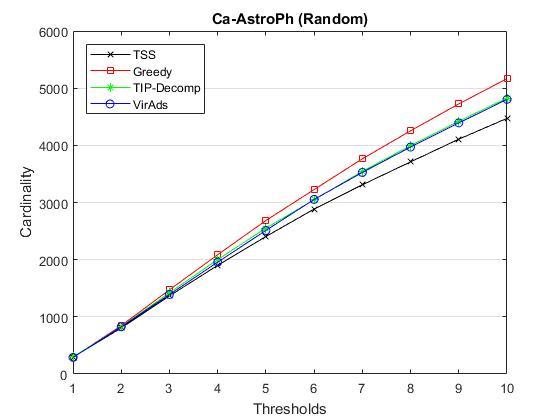
\includegraphics[width=\linewidth,keepaspectratio=true]{images/ca-astrophresultrandom.jpg}
\caption{Time vs Threshold}

\end{minipage}
\begin{minipage}[t]{0.50\textwidth}
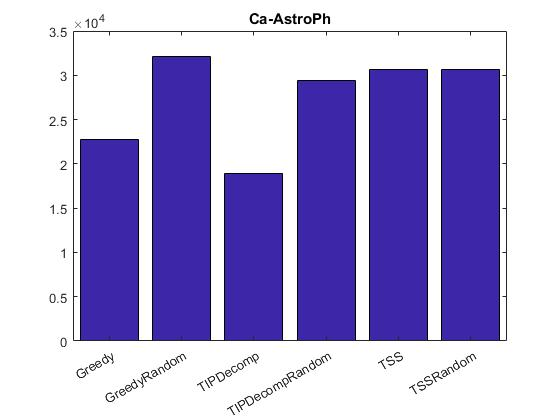
\includegraphics[width=\linewidth,keepaspectratio=true]{images/astrophtime.jpg}
\caption{Time vs Threshold}
\end{minipage}
\end{figure}

\begin{figure}[h!]
\begin{minipage}[t]{0.50\textwidth}
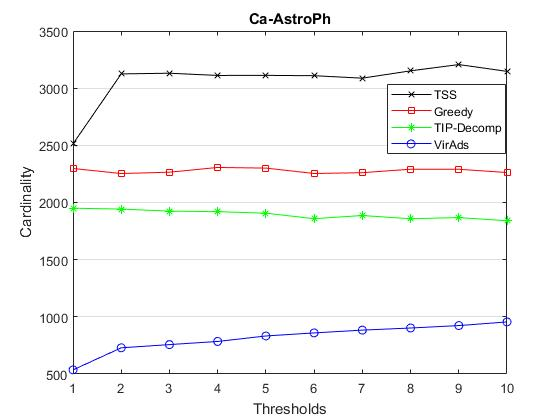
\includegraphics[width=\linewidth,keepaspectratio=true]{images/ca-astrophtime.jpg}
\caption{Time vs Threshold}

\end{minipage}
\begin{minipage}[t]{0.50\textwidth}
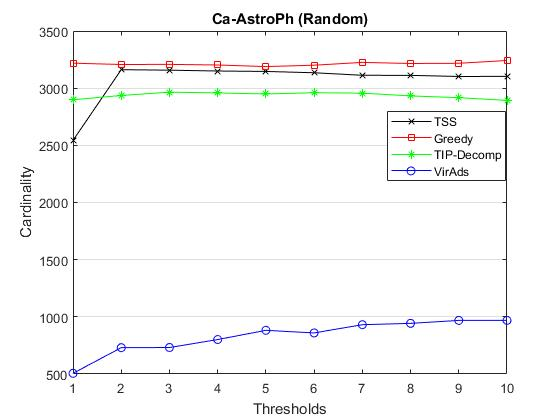
\includegraphics[width=\linewidth,keepaspectratio=true]{images/ca-astrophtimerandom.jpg}
\caption{Time vs Threshold}
\end{minipage}
\end{figure}

\begin{figure}[h!]
\begin{minipage}[t]{0.50\textwidth}
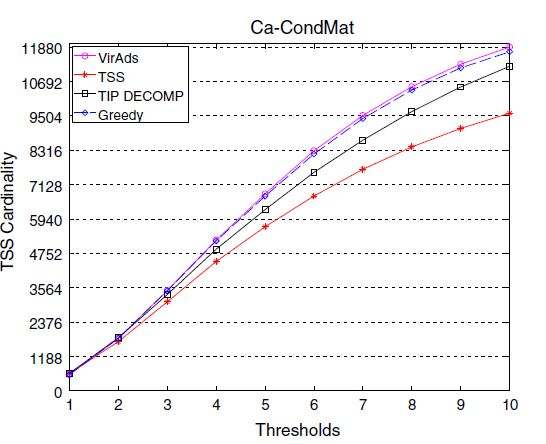
\includegraphics[width=\linewidth,keepaspectratio=true]{images/ca-condmatpaper.jpg}
\caption{Cardinality vs Threshold}

\end{minipage}
\begin{minipage}[t]{0.50\textwidth}
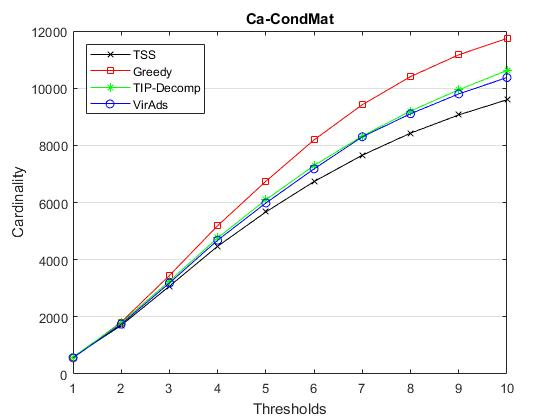
\includegraphics[width=\linewidth,keepaspectratio=true]{images/ca-condmatresult.jpg}
\caption{Cardinality vs Threshold}
\end{minipage}
\end{figure}

\begin{figure}[h!]
\begin{minipage}[t]{0.50\textwidth}
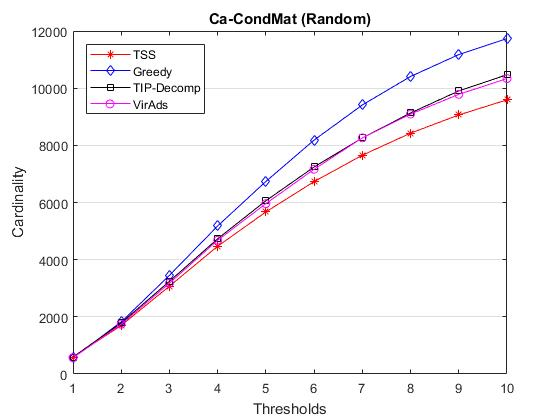
\includegraphics[width=\linewidth,keepaspectratio=true]{images/ca-condmatresultrandom.jpg}
\caption{Time vs Threshold}

\end{minipage}
\begin{minipage}[t]{0.50\textwidth}
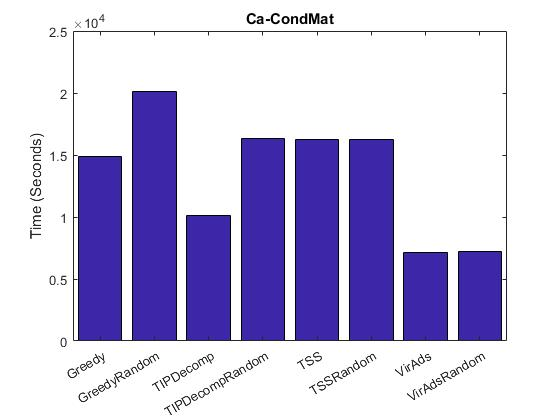
\includegraphics[width=\linewidth,keepaspectratio=true]{images/condmattime.jpg}
\caption{Time vs Threshold}
\end{minipage}
\end{figure}

\begin{figure}[h!]
\begin{minipage}[t]{0.50\textwidth}
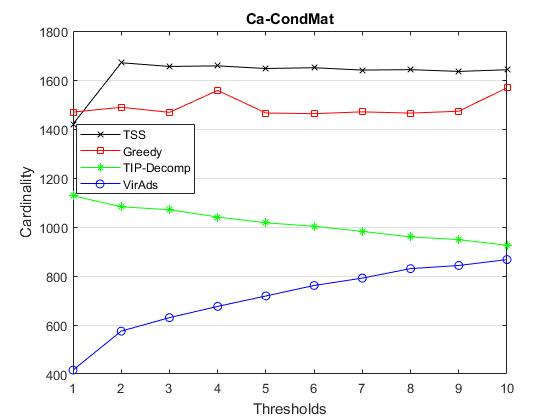
\includegraphics[width=\linewidth,keepaspectratio=true]{images/ca-condmattime.jpg}
\caption{Time vs Threshold}

\end{minipage}
\begin{minipage}[t]{0.50\textwidth}
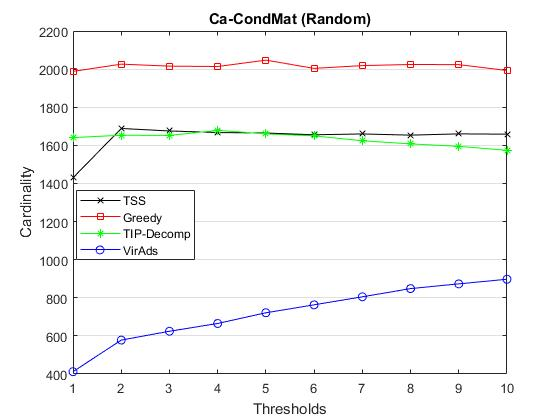
\includegraphics[width=\linewidth,keepaspectratio=true]{images/ca-condmatrandomtime.jpg}
\caption{Time vs Threshold}
\end{minipage}
\end{figure}

\begin{figure}[h!]
\begin{minipage}[t]{0.50\textwidth}
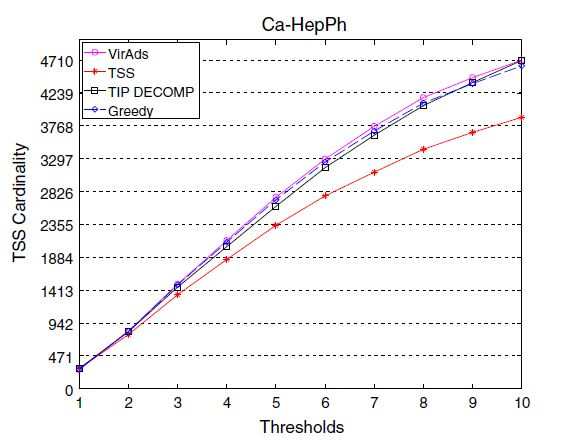
\includegraphics[width=\linewidth,keepaspectratio=true]{images/ca-hepphpaper.jpg}
\caption{Cardinality vs Threshold}

\end{minipage}
\begin{minipage}[t]{0.50\textwidth}
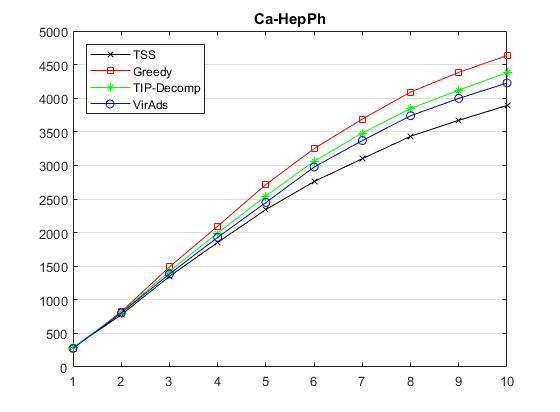
\includegraphics[width=\linewidth,keepaspectratio=true]{images/ca-hepphresult.jpg}
\caption{Cardinality vs Threshold}
\end{minipage}
\end{figure}

\begin{figure}[h!]
\begin{minipage}[t]{0.50\textwidth}
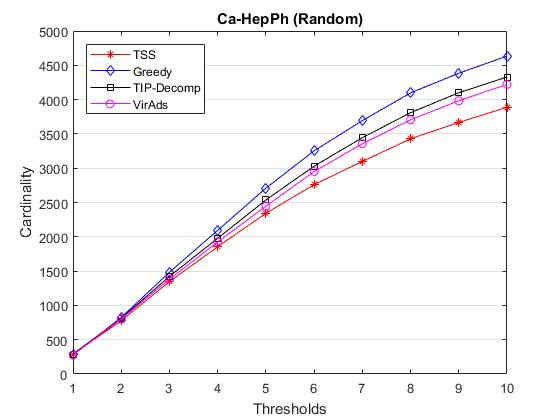
\includegraphics[width=\linewidth,keepaspectratio=true]{images/ca-hepphresultrandom.jpg}
\caption{Time vs Threshold}

\end{minipage}
\begin{minipage}[t]{0.50\textwidth}
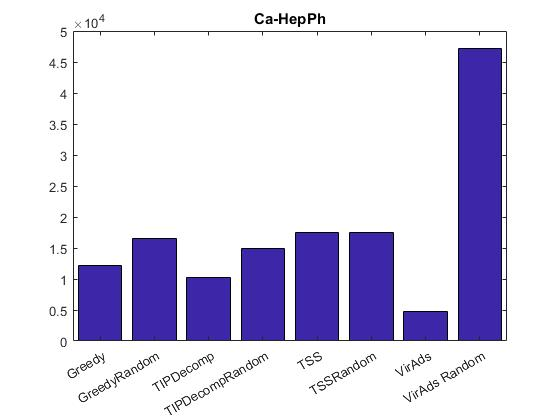
\includegraphics[width=\linewidth,keepaspectratio=true]{images/hepphtime.jpg}
\caption{Time vs Threshold}
\end{minipage}
\end{figure}

\begin{figure}[h!]
\begin{minipage}[t]{0.50\textwidth}
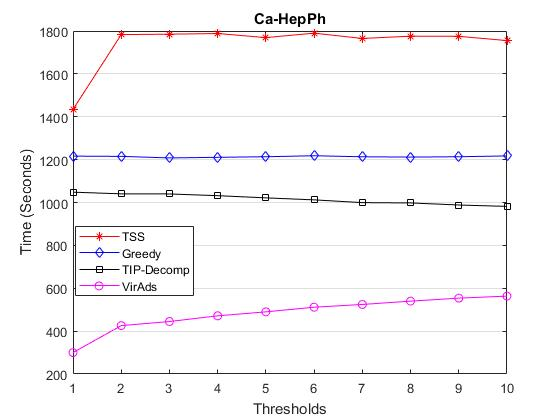
\includegraphics[width=\linewidth,keepaspectratio=true]{images/ca-hepphtime.jpg}
\caption{Time vs Threshold}

\end{minipage}
\begin{minipage}[t]{0.50\textwidth}
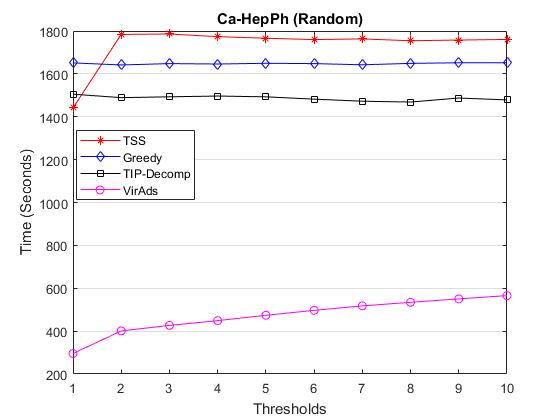
\includegraphics[width=\linewidth,keepaspectratio=true]{images/ca-hepphrandomtime.jpg}
\caption{Time vs Threshold}
\end{minipage}
\end{figure}

\begin{figure}[h!]
\begin{minipage}[t]{0.50\textwidth}
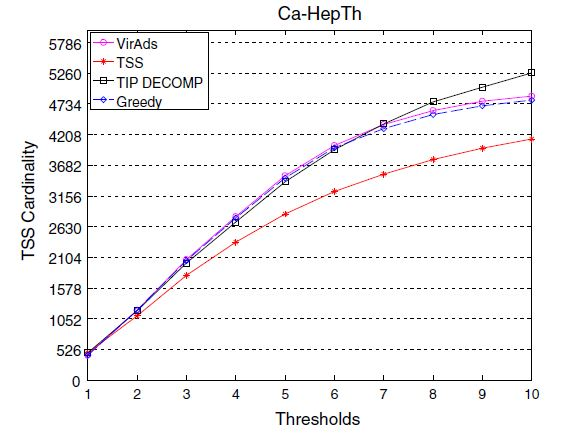
\includegraphics[width=\linewidth,keepaspectratio=true]{images/ca-hepthpaper.jpg}
\caption{Cardinality vs Threshold}

\end{minipage}
\begin{minipage}[t]{0.50\textwidth}
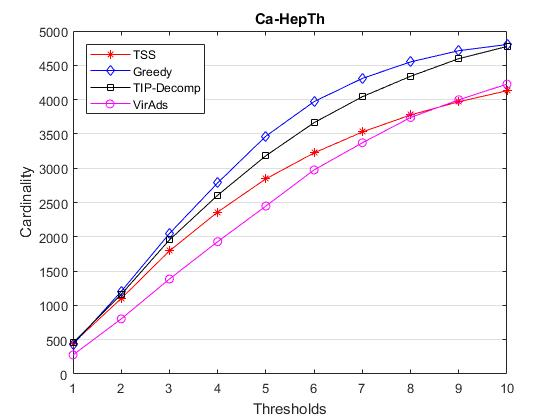
\includegraphics[width=\linewidth,keepaspectratio=true]{images/ca-hepthresult.jpg}
\caption{Cardinality vs Threshold}
\end{minipage}
\end{figure}

\begin{figure}[h!]
\begin{minipage}[t]{0.50\textwidth}
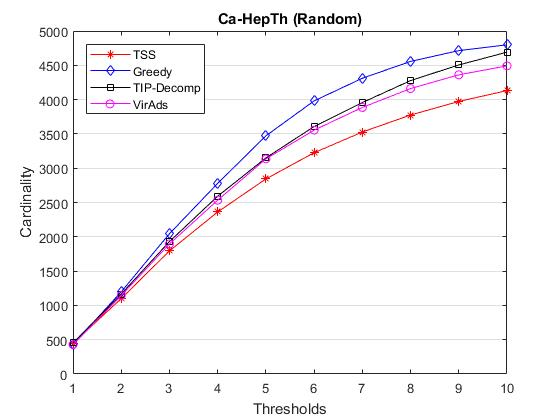
\includegraphics[width=\linewidth,keepaspectratio=true]{images/ca-hepthresultrandom.jpg}
\caption{Time vs Threshold}

\end{minipage}
\begin{minipage}[t]{0.50\textwidth}
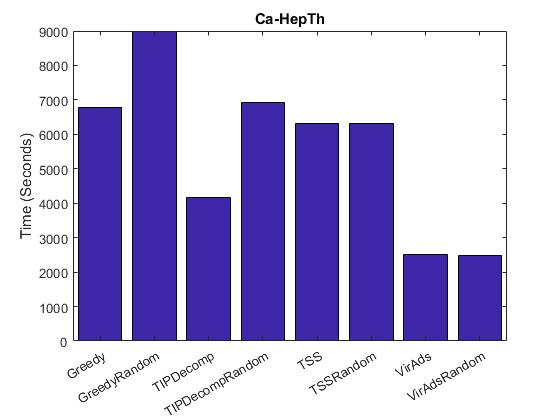
\includegraphics[width=\linewidth,keepaspectratio=true]{images/hepthtime.jpg}
\caption{Time vs Threshold}
\end{minipage}
\end{figure}

\begin{figure}[h!]
\begin{minipage}[t]{0.50\textwidth}
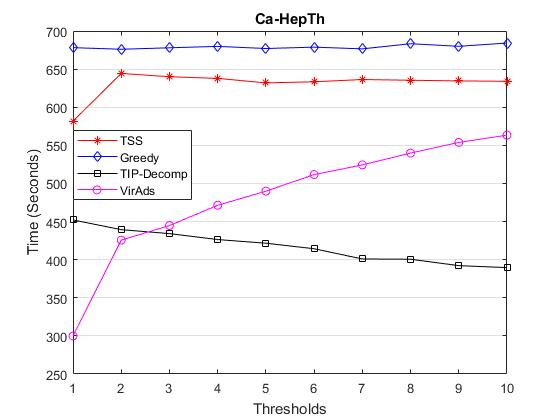
\includegraphics[width=\linewidth,keepaspectratio=true]{images/ca-hepthtime.jpg}
\caption{Time vs Threshold}

\end{minipage}
\begin{minipage}[t]{0.50\textwidth}
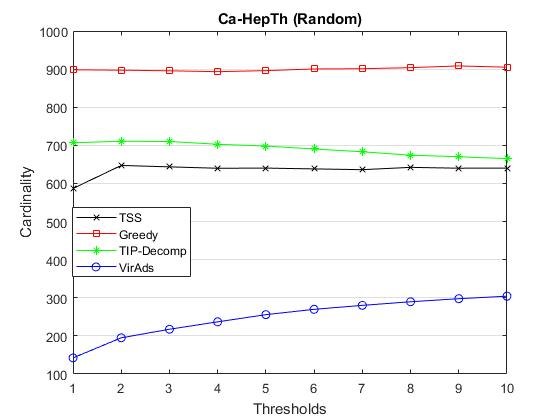
\includegraphics[width=\linewidth,keepaspectratio=true]{images/ca-hepthrandomtime.jpg}
\caption{Time vs Threshold}
\end{minipage}
\end{figure}
	
\begin{figure}[h!]
\begin{minipage}[t]{0.50\textwidth}
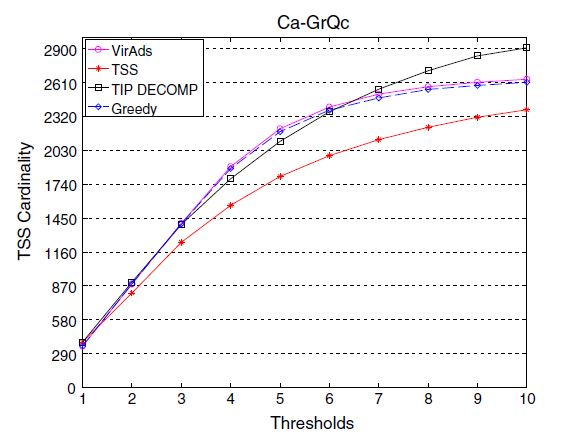
\includegraphics[width=\linewidth,keepaspectratio=true]{images/ca-grqcpaper.jpg}
\caption{Cardinality vs Threshold}

\end{minipage}
\begin{minipage}[t]{0.50\textwidth}
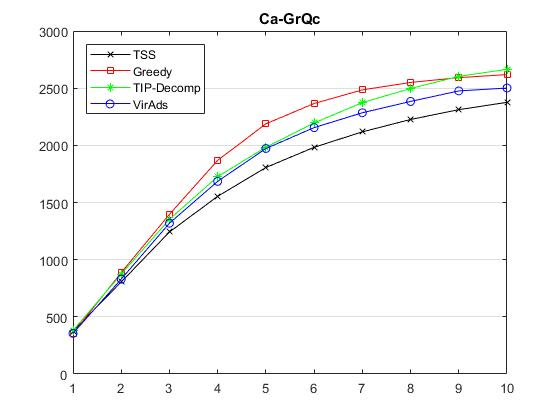
\includegraphics[width=\linewidth,keepaspectratio=true]{images/ca-grqcresult.jpg}
\caption{Cardinality vs Threshold}
\end{minipage}
\end{figure}

\begin{figure}[h!]
\begin{minipage}[t]{0.50\textwidth}
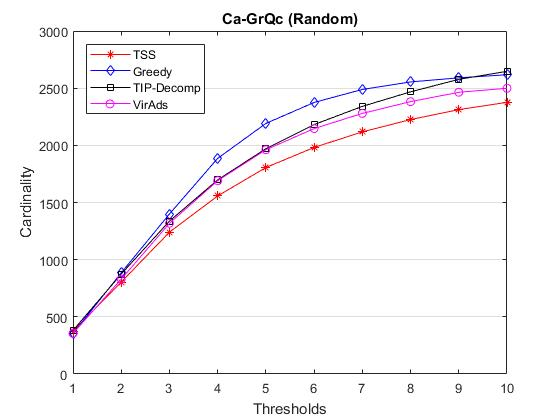
\includegraphics[width=\linewidth,keepaspectratio=true]{images/ca-grqcresultrandom.jpg}
\caption{Time vs Threshold}

\end{minipage}
\begin{minipage}[t]{0.50\textwidth}
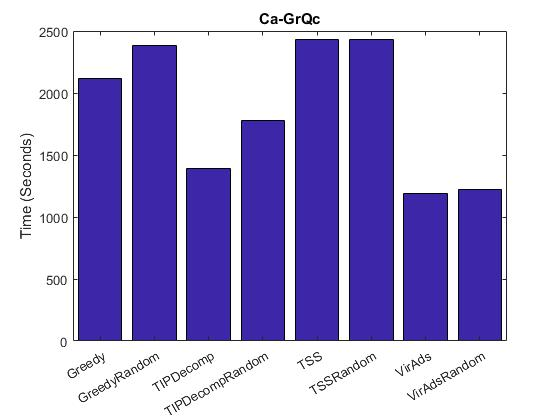
\includegraphics[width=\linewidth,keepaspectratio=true]{images/grqctime.jpg}
\caption{Time vs Threshold}
\end{minipage}
\end{figure}

\begin{figure}[h!]
\begin{minipage}[t]{0.50\textwidth}
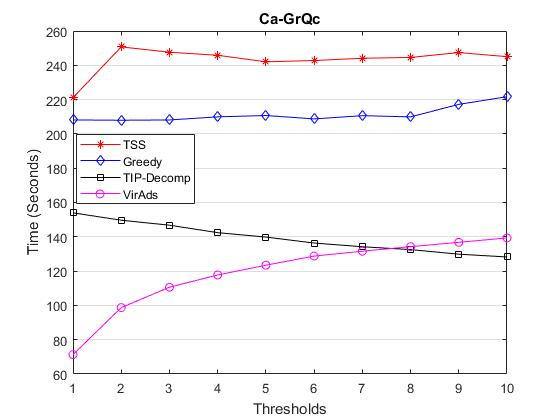
\includegraphics[width=\linewidth,keepaspectratio=true]{images/ca-grqctime.jpg}
\caption{Time vs Threshold}

\end{minipage}
\begin{minipage}[t]{0.50\textwidth}
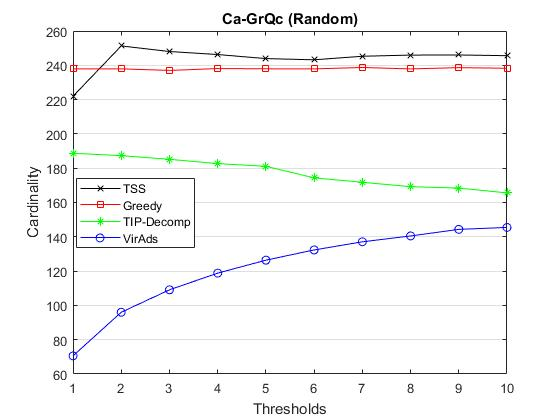
\includegraphics[width=\linewidth,keepaspectratio=true]{images/ca-grqcrandomtime.jpg}
\caption{Time vs Threshold}
\end{minipage}
\end{figure}

\begin{figure}[h!]
\begin{minipage}[t]{0.50\textwidth}
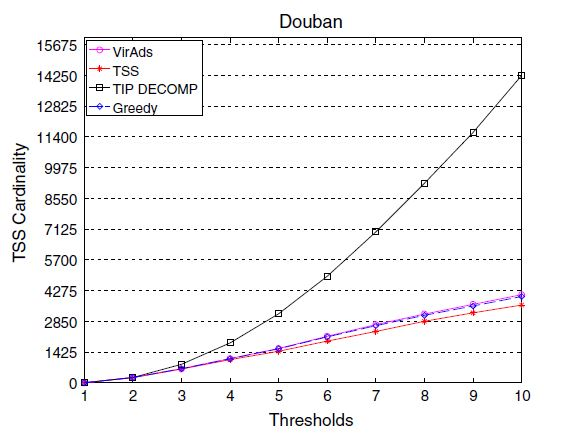
\includegraphics[width=\linewidth,keepaspectratio=true]{images/doubanpaper.jpg}
\caption{Cardinality vs Threshold}

\end{minipage}
\begin{minipage}[t]{0.50\textwidth}
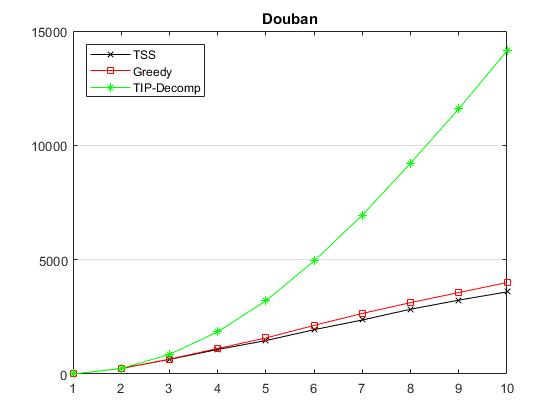
\includegraphics[width=\linewidth,keepaspectratio=true]{images/doubanresult.jpg}
\caption{Cardinality vs Threshold}
\end{minipage}
\end{figure}

\begin{figure}[h!]
\begin{minipage}[t]{0.50\textwidth}
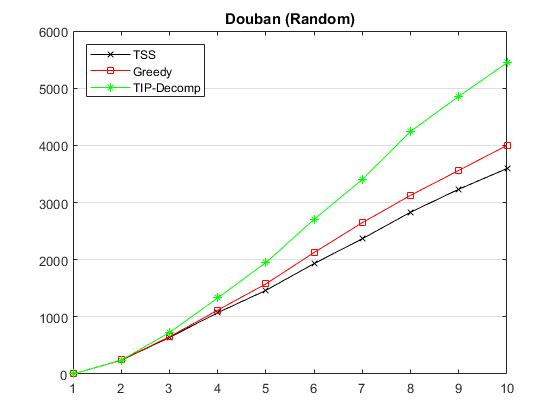
\includegraphics[width=\linewidth,keepaspectratio=true]{images/doubanresultrandom.jpg}
\caption{Cardinality vs Threshold}

\end{minipage}
\begin{minipage}[t]{0.50\textwidth}
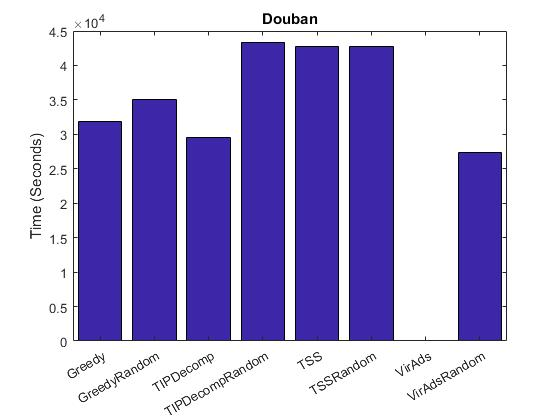
\includegraphics[width=\linewidth,keepaspectratio=true]{images/doubantime1.jpg}
\caption{Time vs Algorithms}
\end{minipage}
\end{figure}

\begin{figure}[h!]
\begin{minipage}[t]{0.50\textwidth}
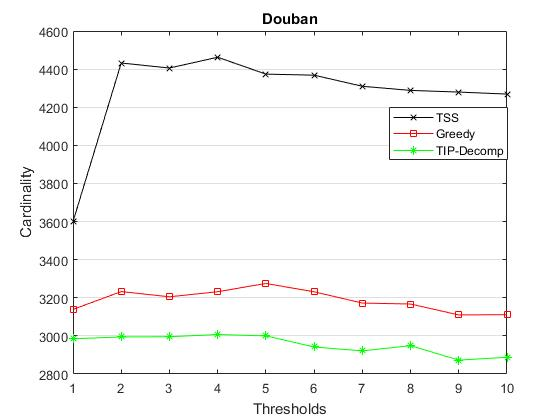
\includegraphics[width=\linewidth,keepaspectratio=true]{images/doubantime.jpg}
\caption{Time vs Threshold}

\end{minipage}
\begin{minipage}[t]{0.50\textwidth}
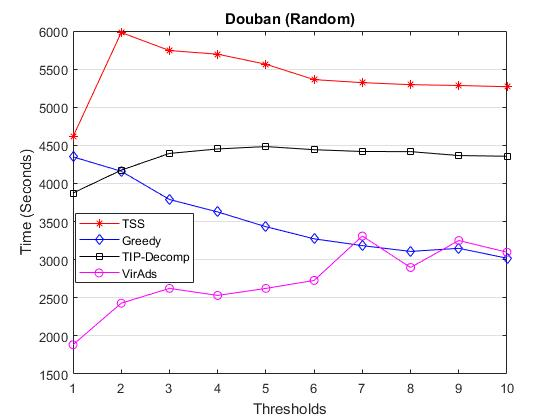
\includegraphics[width=\linewidth,keepaspectratio=true]{images/doubantimerandom.jpg}
\caption{Time vs Threshold}
\end{minipage}
\end{figure}

From the graphs we can observe that for the majority of our graphs, the TSS algorithm obtains the least cardinality for every thresholds.

The time versus thresholds graphs show that in TSS we obtain fastest result when all the vertices' thresholds is 1. Note that with $t=1$, most of the time we go to case 1($t=0$) of the algorithm just after the first removal of the first node. This implies a fast computation of the equation in case 3($\frac{t(v)}{d(v)(d(v)+1}$). At the end there remains a single node (for some datasets it is more than 1) that has its degree to be less than its threshold, meaning we need to include it to the target set. VirAds seems to be the only algorithm to show that as the threshold increases, so does the time it takes to obtain the target set. The other algorithms seem to show that the time it takes per threshold is somewhat \textit{constant} through out the thresholds.

The bar plots comparing the algorithms shows that the TSS took the longest time in finding the target set. This maybe due to the fact that in our code we update a property of a node every iteration to keep track of the selection of nodes in case 3. In the paper, Cordasco did not report the run times of the experiment, stating that this experiment is very machine and implementation dependent.